\appendix
\label{Anhang}
\section{Anhang}

\subsection{Weitere Aktivierungsfunktionen}\label{anhang:weitereaktivierungsfunktionen}

\begin{figure}[h]
    \center
    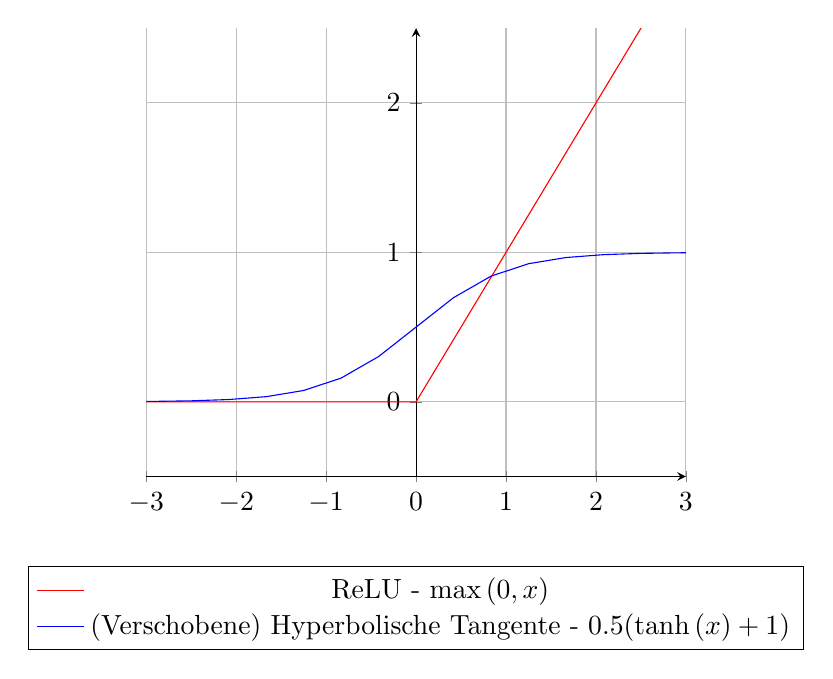
\begin{tikzpicture}
    \begin{axis}
        [
            grid=major,
            xmin=-3,
            xmax=3,
            axis x line=bottom,
            ytick={0,1,2},
            ymax=2.5,
            ymin=-0.5,
            axis y line=middle,
            legend style={at={(0.5,-0.2)},anchor=north}
        ]
        \addplot[red,mark=none]{(x>=0)*x};
        \addplot[blue, mark=none]{0.5*(tanh(\x)+1)};
        \legend{ReLU - $\max{(0,x)}$, (Verschobene) Hyperbolische Tangente - $0.5(\tanh{(x)}+1)$}
    \end{axis}
\end{tikzpicture}
    \caption[Aktivierungsfunktionen]{Weitere Aktivierungsfunktionen, ergänzend zu der Sigmoid Funktion aus Kapitel \ref{funktionsweise}}
    \label{Aktivierungsfunktionen}%
\end{figure}

Die ReLU (Rectified linear Unit) Funktion ist im Vergleich zu anderen Aktivierungsfunktionen, wie der Sigmoidfunktion oder der Hyperbolischen Tangente, deutlich simpler, was sich in Leistungsansprüchen des Trainingsprozesses wiederspiegelt.\footnote{\cite{nnfs}}

\subsection{Code für das Beispiel aus \ref{funktionsweise}}\label{anhang:colab1}

\begin{listing}[H]
    \begin{minted}[fontsize=\scriptsize,linenos]{python}
import tensorflow as tf
import tensorflow.keras.layers as layers

numberOfNeuronsInFirstLayer = 16 
numberOfNeuronsInSecondLayer = 16 
numOfEpochs = 5 

mnist = tf.keras.datasets.mnist

(x_train, y_train), (x_test, y_test) = mnist.load_data() # Laden des MNIST Datasets
# Und aufteilen in Trainigsdaten und Testdaten

x_train = tf.keras.utils.normalize(x_train, axis=1) # Normalisieren des Datasets
x_test = tf.keras.utils.normalize(x_test, axis=1)

model = tf.keras.models.Sequential() # Erstellen des Neuronalen Netzwerks
model.add(layers.Flatten())
model.add(layers.Dense(numberOfNeuronsInFirstLayer, activation=tf.nn.sigmoid))
# Hinzufügen der Layer
model.add(layers.Dense(numberOfNeuronsInSecondLayer, activation=tf.nn.sigmoid))
model.add(layers.Dense(10, activation=tf.nn.softmax))

model.compile(optimizer='adam',
              loss='sparse_categorical_crossentropy',
              metrics=['accuracy']) # Kompilieren der Layer zu einem trainierfähigen Modell

model.fit(x_train, y_train, epochs=numOfEpochs)
# Trainieren des Modells mit den Trainingsdaten und x Epochen

model.save('beispielModel_MNIST') # Speichern des Modells

    \end{minted}
    \caption{Umsetzung mit Python und Tensorflow}
\end{listing}
Ein Interaktives Beispiel gibt zusätzlich es hier in meinem Colab Notebook: \url{https://bit.ly/34Ggfuh}\footnote{Ungekürzter Link: \url{https://colab.research.google.com/drive/1ty_QQlL038YT6KpBjSdqGvIGyH0YXwxW}}